\documentclass[60x84/16,8pt]{ittmm}

\usepackage[T1,T2A]{fontenc}
\usepackage{ucs}
\usepackage[utf8x]{inputenc}
\usepackage[english,russian]{babel}

%% Расширенная математика

\usepackage{amsmath}
\usepackage{amssymb}
\usepackage{amscd}

\usepackage{mathtools}
\mathtoolsset{
showonlyrefs=true,
mathic=true,
}

\allowdisplaybreaks

%% Работа с графикой

\usepackage{graphicx}

%% hyperref

\usepackage{hyperref}
\hypersetup{backref,
 colorlinks=false}
\hypersetup{pdfborder=0 0 0}

%% local definitions

\geometry{twoside}
\geometry{bindingoffset=0pt}

\geometry{includehead}
\geometry{hmargin={16mm,16mm},vmargin={12mm,13mm}}
\geometry{marginparwidth=0pt,marginparsep=0pt}
\geometry{headheight=0pt}
\geometry{headsep=\baselineskip}

\pagestyle{empty}

\usepackage{cite}

\makeatletter
\g@addto@macro\@maketitle@hook@post{%
 \iflanguage{english}{%
   \bibliographystyle{elsarticle-num}
 }{%
   \bibliographystyle{ugost2008l}
 }
}
\makeatother

%%% Local Variables:
%%% mode: latex
%%% coding: utf-8-unix
%%% End:


\begin{document}

% Укажите индекс УДК, соответствующий Вашей работе.
% Рукопись должна содержать УДК, который рекомендуется брать из следующего источника: \url{http://www.mathnet.ru/udc.pdf}.
\udc{004.8}

\title{Разработка и исследование модели для генерации субъективно привлекательных лиц людей}

\author[1]{М. А. Ким}

\address[1]{Кафедра математического моделирования и искусственного интеллекта,\\
  Российский университет дружбы народов,\\
  ул. Миклухо-Маклая, д.6, Москва, Россия, 117198}

\email{\url{1032201664@pfur.ru}}

\begin{abstract}
Когнитивные способности человека позволяют осуществлять восприятие, анализ и внешнюю оценку собеседника.
При этом объяснение субъективной оценки внешности нельзя назвать тривиальной задачей.
Помимо известных общих закономерностей, таких как принципы геометрии лица, а также социальный и культурный опыт оценивающего,
каждому человеку присуще комплексные индивидуальные факторы, влияющие на субъективное понимание красоты.
Настоящая статья посвящена задаче построения модели машинного обучения, способной в соответствии с обратной связью
от пользователя генерировать субъективно привлекательные лица людей.
Предполагается, что такая модель поможет в изучении процесса формирования человеком оценки привлекательности лиц
и выявлении индивидуальных факторов, влияющих на данный показатель. В работе рассмотрено программное обеспечение,
предоставляющее пользователю возможность последовательного выбора и оценки по заданному показателю качества наиболее
привлекательных изображений из набора, созданного при помощи модели машинного обучения.
По окончании заданной длины последовательности изображений пользователю предоставляется возможность
оценить результирующее изображение на предмет привлекательности лица.
Средняя оценка выбранных в наборе изображений сравнивается с оценкой результирующего изображения.
В статье даются выводы о качестве генерации изображений по мнению пользователей и о возможностях применения полученных результатов.
\end{abstract}

\keywords{изображения лиц, визуализация, генеративные состязательные сети, машинное обучение}

\alttitle{Development and research of a model for generating subjectively attractive human faces}

\altauthor[1]{M. A. Kim}

\altaddress[1]{Department of Information Technologies\\
Peoples' Friendship University of Russia\\
Miklukho-Maklaya str. 6, Moscow, 117198, Russia}

\begin{altabstract}
A person's cognitive abilities enable perception, analysis, and external evaluation of the interlocutor.
At the same time, the subjective assessment of attractiveness cannot be considered a trivial task.
In addition to well-established general patterns, such as facial geometry principles, as well as social and cultural experiences of the evaluator,
each person has complex individual factors that influence subjective understanding of beauty.
This article aims to develop a machine learning model that can utilize feedback from the user
to produce subjectively attractive faces. It is assumed that such a model would assist in examining
the formation of a person's evaluation of attractiveness and identifying individual factors influencing
this indicator. This paper discusses software that provides the user with an opportunity to consistently
select and evaluate the most attractive individuals.Attractive images generated using a machine learning
model based on a given quality metric. At the end of a specified sequence of images, users are given the
opportunity to evaluate the facial attractiveness of the final image. The average score of images selected
from the set is then compared to the score of the generated image. The article concludes on the basis of user
feedback and the potential applications of the generated results.
\end{altabstract}

\altkeywords{face images, visualization, generative adversarial networks, machine learning}

\maketitle

\section{Введение}
\label{sec:intro}

Человек обладает способностью классифицировать привлекательность и степень
красоты заданного объекта по его изображению.
Однако, в большинстве случаев, невозможно произвести количественную оценку избранного решения.
Особенно остро данный аспект проявляется при анализе и генерации человеческих лиц.

Трудности исследования данного направления связаны в первую очередь с тем, что
оценка привлекательности одного и того же объекта разными людьми может сильно различаться
в виду, к примеру, возраста, культуры и пола оценивающего
\cite{facial-attractiveness-1, facial-attractiveness-2, facial-attractiveness-3}.
Считается, что есть и общие закономерности, связывающие определенные черты лица
и среднюю оценку его привлекательности, такие как его симметричность, приблизительно
равная соотношению носа ко лбу и носа к подбородку \cite{facial-attractiveness-math-1}.
Однако, в общем случае, привлекательность -- скорее субъективная, личностная характеристика,
нежели объективный фактор, справедливый для большинства людей.

Создание визуально привлекательных изображений людей до сих пор
является является сложной задачей в виду затруднительности описания
оценки качества ее решения. Большинство исследований в данной области
направлены на выявление определенных закономерностей лица в соответствии
с его фотографией \cite{facial-attractiveness-math-2, facial-attractiveness-math-3, facial-attractiveness-math-4},
однако, вероятно, подходы такого рода не позволяют выявить все
факторы, влияющие на субъективную оценку в виду сложности человеческих суждений
относительно привлекательности. Модели, создающие изображения на основе выявленных
зависимостей, не способны полностью отразить эстетическое восприятие человека \cite{attr-models-complicated}.
Это связанно с тем, что генерация объектов ограниченна заданными
общими закономерностями и не учитывает субъективные предпочтения человека.

В данной статье представлен альтернативный метод создания субъективно привлекательных
изображений лиц людей на основе генеративно-состязательной нейронной сети (GAN) \cite{gan},
обученной на датасете CelebA-HQ \cite{celeba-hq}.
Коррекция в генерации лиц в соответствии с предпочтениями человека производится
на основе анализа скрытого пространства (latent space) нейронной сети \cite{latent-space-exploration}. 

\section{Построение модели} 
\label{sec:base-section}

Предлагаемая архитектура модели представляет собой сверточную
генеративно-состязательную сеть глубокого обучения (DCGAN) \cite{dcgan}.
DCGAN является прямым продолжением развития архитектуры GAN: модель также 
состоит из двух нейронных сетей, генератора и дискриминатора, обучаемых независимо друг от друга.
Генератор создает изображения, основываясь на векторе случайных чисел с плавающей точкой,
генерируемых в соответствии с нормальным распределением. Дискриминатор дает оценку поступающим
реальным и сгенерированным изображениям. Критерии качества для генератора и дискриминатора задаются согласно
бинарной кроссэнтропии и представляются формулами \eqref{eq:loss_dis}, \eqref{eq:loss_gen}.

\begin{equation}
  loss\_dis=-\log(real) - \log(1-fake)
  \label{eq:loss_dis}
\end{equation}

\begin{equation}
  loss\_gen=-\log(fake),
  \label{eq:loss_gen}
\end{equation}

где \(fake \in [0, 1]\) --- уверенность дискриминатора в генеративной природе изображения,
\(real \in [0, 1]\) -- уверенность дискриминатора в том, что изображение является настоящим.

В представленных моделях генератор и дискриминатор соревнуются, что приводит
к увеличению качества генерируемых изображений при увеличении числа эпох и
при условии обеспечения сходимости модели. Архитектура DCGAN изменяет классическую архитектуру GAN,
добавляя сверточные слои Convolutional и Convolutional Transpose в генератор и дискриминатор.
Данная модификация позволяет улучшить качество результирующих изображений при использовании
множества скрытых слоев в нейронной сети.

Возможность использования векторной арифметики
в скрытом пространстве генератора позволяет создавать новые изображения на основе усреднения
векторов скрытого состояния целевых изображений, генерируя тем самым лица,
совмещающие в себе черты целевых изображений.

\section{Обучение модели}
\label{sec:base-section}

Обучение модели производилось на датасете CelebA-HQ,
который содержит 30000 изображений лиц знаменитостей с разрешением 1024×1024px.
Для обучения модели использовались изображения,
представляющие из себя набор пикселей в формате RGB. При этом метаинформация, такая как именование
различных признаков на изображении, не использовалась при обучении.
Разрешение изображений было понижено до 128x128px перед обучением.
Обучение производилось на протяжении 50 эпох. Результирующая кривая
обучения для генератора и дискриминатора представлена на рис. \ref{fig:learning-curve}.

\begin{figure}
  \centering
  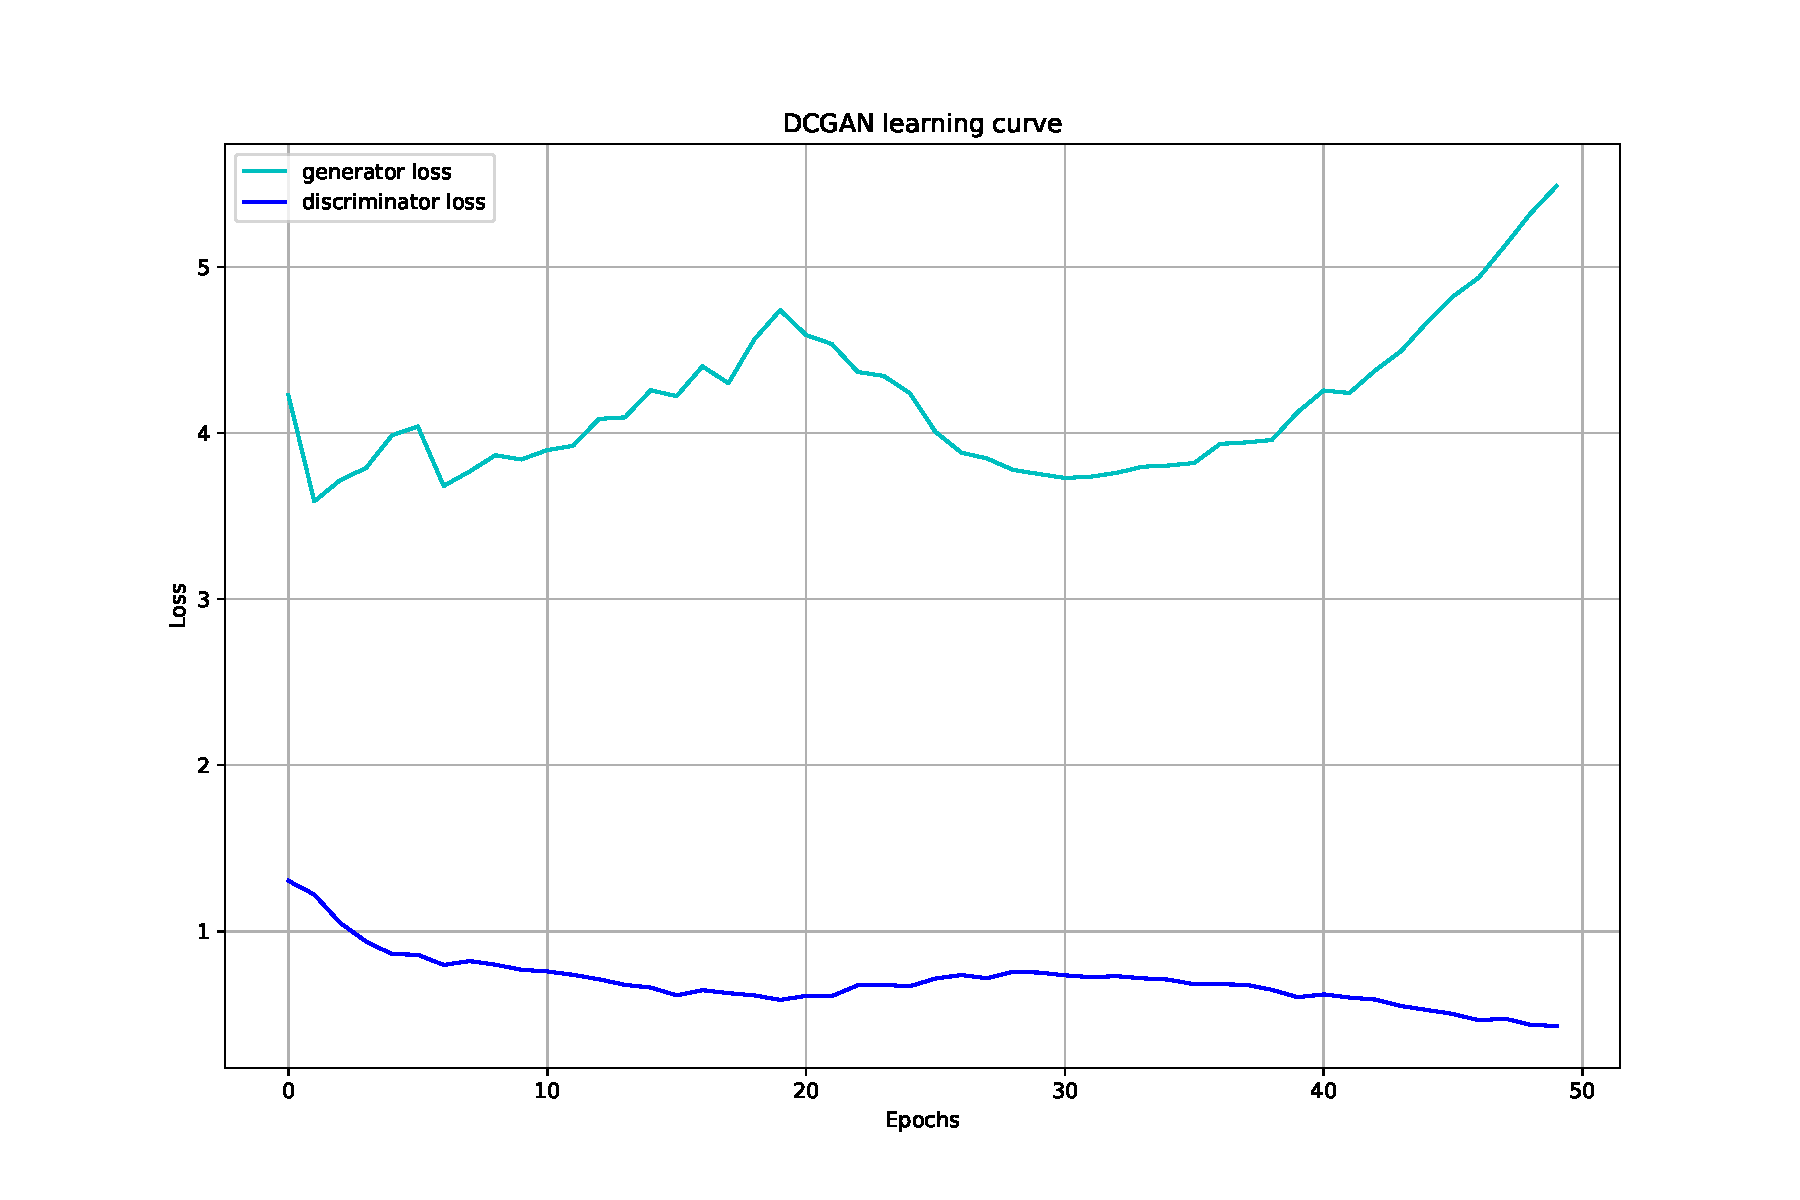
\includegraphics[width=\linewidth]{learning_curve}
  \caption{Кривая обучения}
  \label{fig:learning-curve}
\end{figure}

\section{Внедрение и оценка модели}
\label{sec:base-section}

Примеры генерации лиц со скрытым пространством, заполненным случайно в соответствии с нормальным распределением,
показаны на рис. \ref{fig:result-random-seed}.

\begin{figure}
  \centering
  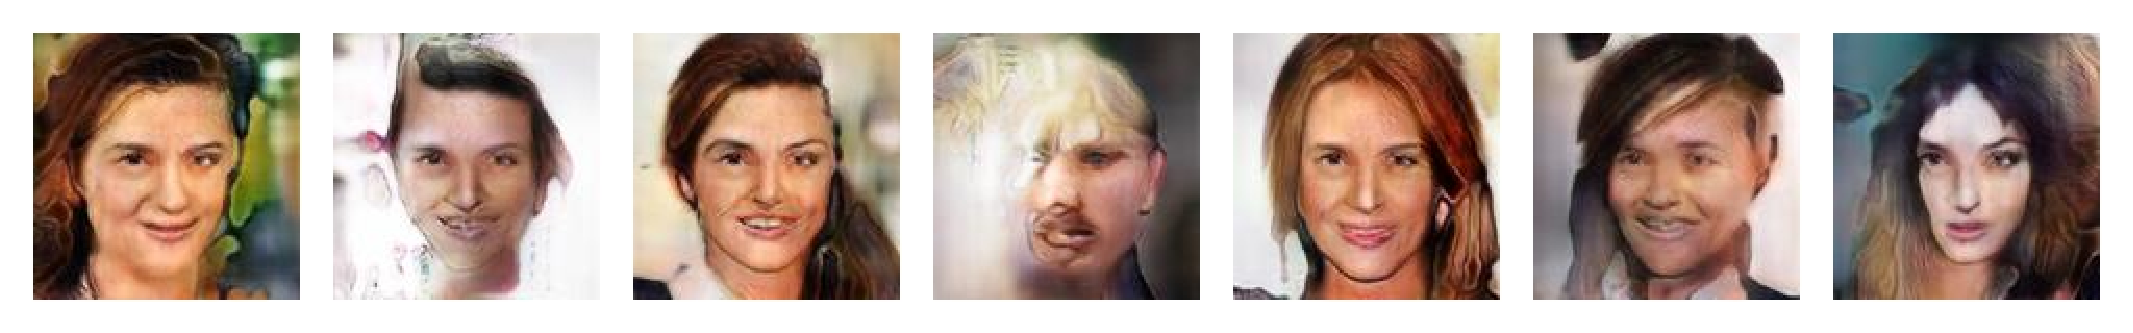
\includegraphics[width=\linewidth]{output}
  \caption{Примеры генерации лиц со случайным SEED}
  \label{fig:result-random-seed}
\end{figure}

Пример усреднения вектора скрытого пространства показан на рис. \ref{fig:interpolation}, где изображение слева
получено путем усреднения векторов скрытого пространства остальных изображений.

\begin{figure}
  \centering
  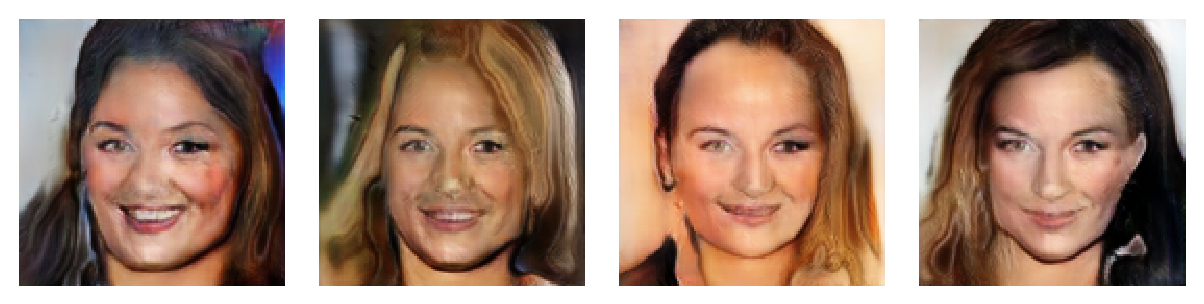
\includegraphics[width=0.8\linewidth]{interpolation}
  \caption{Усреднение векторов скрытого пространства}
  \label{fig:interpolation}
\end{figure}

Предположение, выдвигаемое настоящей статьей, полагает, что при выборе участником исследования
нескольких субъективно привлекательных изображений и усреднении их векторов скрытых
пространств в виде нового вектора, можно сгенерировать изображение,
являющееся более привлекательным для участника исследования по сравнению с избранными ранее
изображениями.

Для проверки предположения была выбрана стратегия, заключаящаяся в последовательном показе набора из четырех
случайно сгенерированных изображений три раза. В каждом наборе пользователю предлагалось выбрать
наиболее привлекательное изображение и оценить степень его привлекательности по шкале от 1 до 10
(где 1 -- наиболее отталкивающее возможное изображение, 10 -- наиболее привлекательное возможное изображение).
На основе векторов скрытых состояний трех полученных изображений строилось результирующее изображение,
которое оценивалось пользователем по заданной выше системе оценки.

Был проведен эксперимент с участием 20 человек (\(N = 20\)).
Результат эксперимента представлен в табл. \ref{tab:experiment},
где \(avg(T)\) -- средняя оценка изображений, выбранных из наборов участником,
\(T^r\) -- оценка сгенерированного итогового изображения.

\begin{table}
  \centering
  \caption{Результат исследования}
  \label{tab:experiment}
  \begin{tabular}{|c|c|}
    \hline
    \(\delta (avg(T), T^r)\) & Число участников \(n \in N\) \\
    \hline
    \(\ge 2\) & 2 \\
    1         & 9 \\
    0         & 3 \\
    -1        & 2 \\
    \(\le -2\)& 4 \\
    \hline
  \end{tabular}
\end{table}

Результат исследования показывает, что 55\% участников посчитали результирующее
изображение более привлекательным, нежели выбранные из наборов.
При этом 30\% пользователей оценили итоговое изображение, как
непривлекательное по сравнению с начальными.

При оценке результатов стоит брать во внимание тот факт, что
построенная модель на базе DCGAN не способна генерировать
реалистичные лица людей: пропорции не всегда соблюдены верно,
изображения содержат артефакты. По данной причине при проведении
исследования его участниками отмечалось, что предоставленные изображения
лиц не похожи на настоящии фотографии людей. В следствии этого,
нельзя назвать выдвигаемую гипотезу доказанной, не смотря на тот факт,
что исследование показывает некоторый положительный результат.

Для последующего доказательства гипотезы следует использовать
значительно более сложные предобученные модели машинного обучения
по типу StyleGAN3 \cite{stylegan} и Stable Diffusion \cite{sd}, что позволит генерировать
действительно фотореалистичные изображения лиц людей, а также
предоставит большую возможность в исследовании влияния вектора скрытого
пространства модели.

\section{Заключение}

В настоящей работе рассмотрен метод генерации субъективно привлекательных лиц людей
путем усреднения векторов скрытого пространства сверточной
генеративно-состязательной сети глубокого обучения. Дальнейшее исследование скрытого пространства
может помочь в выявлении комплексных факторов, влияющих на субъективную
оценку внешности человеком.

По результатам исследования можно сделать вывод в необходимости
использования более сложных моделей нейронных сетей для решения
поставленной проблемы в связи с неспособностью DCGAN генерировать
фотореалистичные лица людей. Планируется проведение дальнейших исследований
с использованием предобученных моделей StyleGAN3 и Stable Diffusion
для улучшения качества генерации изображений.


\begin{thebibliography}{99}

\bibitem{facial-attractiveness-1}
M. R. Cunningham, A. R. Roberts, A. P. Barbee, P. B. Druen and C.-H. Wu.
Their ideas of beauty are on the whole the same as ours. 
--- Vol. 68, no. 2.

\bibitem{facial-attractiveness-2}
J. H. Langlois, J. M. Ritter, L. A. Roggman and L. S. Vaughn.
Facial diversity and infant preferences for attractive faces. 
--- Vol. 27, no. 1.

\bibitem{facial-attractiveness-3}
R. Thornhill and S. W. Gangestad.
Facial attractiveness. 
--- Vol. 3, no. 12. 
--- P. 452-460.

\bibitem{facial-attractiveness-math-1}
K. Schmid, D. Marx and A. Samal.
Computation of a face attractiveness index based on neoclassical canons, symmetry, and golden ratios. 
--- Vol. 41, no. 8.

\bibitem{facial-attractiveness-math-2}
A. C. Little, B. C. Jones and L. M. DeBruine.
Facial attractiveness: Evolutionary based research. 
--- Vol. 366, no. 1571.
--- P. 1638-1659.

\bibitem{facial-attractiveness-math-3}
D. Perrett, K. A. May and S. Yoshikawa.
Facial shape and judgements of female attractiveness.
--- Vol. 368.
--- P. 239-242.

\bibitem{facial-attractiveness-math-4}
J. Shi, A. Samal and D. Marx.
How effective are landmarks and their geometry for face recognition?. 
--- Vol. 102, no. 2.
--- P. 117-133.

\bibitem{attr-models-complicated}
M. Ibáñez-Berganza, A. Amico and V. Loreto.
Subjectivity and complexity of facial attractiveness. 
--- Vol. 9, no. 1.
--- P. 1-12.

\bibitem{gan}
I. Goodfellow et al..
Generative adversarial nets. 
--- P. 2672-2680.

\bibitem{latent-space-exploration}
Huiting Yang, Liangyu Chai, Qiang Wen, Shuang Zhao, Zixun Sun and Shengfeng He.
Discovering interpretable latent space directions of gans beyond binary attributes. 
--- Vol. 33.

\bibitem{dcgan}
A. Radford, L. Metz, S. Chintala.
Unsupervised Representation Learning with Deep Convolutional Generative Adversarial Networ. 
--- P. 31-38.

\bibitem{celeba-hq}
Tero Karras, Timo Aila, Samuli Laine, Jaakko Lehtinen [Электронный ресурс].
Papers With Code, 2021.
См. URL: https://paperswithcode.com/dataset/celeba-hq

\bibitem{stylegan}
Tero Karras and Miika Aittala and Samuli Laine and Erik H\"ark\"onen and Janne Hellsten and Jaakko Lehtinen and Timo Aila [Электронный ресурс].
Alias-Free Generative Adversarial Networks (StyleGAN3)

\bibitem{sd}
Robin Rombach, Andreas Blattmann, Dominik Lorenz, Patrick Esser, Björn Ommer.
High-Resolution Image Synthesis with Latent Diffusion Models

\end{thebibliography}


% Возможно использовать bibtex.
% Который не работает. Ага, спасибо...
% \bibliographystyle{ugost2008l}
% \bibliography{main}

\makealttitle

\end{document}
